
\documentclass[
11pt, % The default document font size, options: 10pt, 11pt, 12pt
%oneside, % Two side (alternating margins) for binding by default, uncomment to switch to one side (for drafting/reading purposes)
%english, % english for English;
portuguese,% for Portuguese; delete temporary files if you change language (e.g. 'make clean; make')
singlespacing, % Single line spacing, alternatives: onehalfspacing or doublespacing (for drafting/reading purposes)
%draft, % Uncomment to enable draft mode (no pictures, no links, overfull hboxes indicated)
%nolistspacing, % If the document is onehalfspacing or doublespacing, uncomment this to set spacing in lists to single
liststotoc, % Uncomment to add the list of figures/tables/etc to the table of contents (recommended)
%toctotoc, % Uncomment to add the main table of contents to the table of contents (not recommended)
parskip, % Add space between paragraphs (recommended)
%nohyperref, % Uncomment to not load the hyperref package (not recommended)
nohyperreflinkcolor, % hyperref links are not colored (comment to color links, for example to produce an electronic-only version)
headsepline, % Uncomment to get a line under the header
]{tmdei-style} % The class file specifying the document structure

\usepackage{tikz} % Required for creating graphics programmatically (can be removed if not used)
%\usetikzlibrary{arrows} % Required for fancy arrows in TiKZ graphics (can be removed if not used)

\usepackage{pgfplots} % Required for drawing high--quality function plots (can be removed if not used)
\pgfplotsset{compat=newest}

\usepackage[style=authoryear-comp,backend=biber]{biblatex} 

\addbibresource{mainbibliography.bib} % The filename of the bibliography

\usepackage[acronym]{glossaries} % Load glossaries package
\makeglossaries % build the glossary

%----------------------------------------------------------------------------------------
%	THESIS INFORMATION
%----------------------------------------------------------------------------------------

\thesistitle{Desenvolvimento de uma plataforma de gestão de projetos} % Your thesis title, this is used in the title, print it elsewhere with \ttitle

%\thesissubtitle{{[}Thesis Subtitle{]}} % Your thesis title, this is used in the title, print it elsewhere with \tsubtitle

\author{Carlos Santos} % Your name, this is used in the title page, print it elsewhere with \authorname

\subjectarea{Engenharia de Software} % Specialisation area (Cybersecurity and Systems Administration; Data Engineering; Software Engineering;Games, Graphics and Interactive Systems; Information and Knowledge Systems), used in the title page, print it elsewhere with \areaname

\advisor{Professor Nuno Escudeiro} % Your advisors's (academic mentor) name, this is used in the title page, print it elsewhere with \advname

%\coadvisor{Dr. Jack \textsc{Smith}} % Your co-advisors's name, this is used in the title page, print it elsewhere with \coadvname (comment, if no co-advisor)

%\cosupervisor{Dr. Jack \textsc{Smith}} % Your co-advisors's name, this is used in the title page, print it elsewhere with \cosupname (comment, if no co-supervisor)

% if committeepresident is defined, will add the thesis committee to the front page
%\committeepresident{Dr. Jonny Smith, Professor, DEI/ISEP} % Name of the president of the evaluation committee, print it elsewhere with \presidentname

%\committeemembers{Dr. Jaimie Smith, Professor, DEI/ISEP\\Dr. Jones Smith, Professor, DEI/ISEP\\Dr. Jagger Smith, Professor, DEI/ISEP} % Name of the evaluation committee members (up to four), print it elsewhere with \committee

\keywords{Frontend, Backend, Software Architecture, } % Please define up to 6 keywords that better describe your work, print it elsewhere with \keywordnames

\university{\href{http://www.university.com}{University Name}} % Your university's name and URL, this is used in the title page and abstract, print it elsewhere with \univname

\department{\href{http://dei.isep.ipp.pt}{Departamento de Engenharia Informatica}} % Your department's name and URL, this is used in the title page and abstract, print it elsewhere with \deptname

\thesisdate{Porto, Setembro, 2025} % thesis date,  print it elsewhere with \tdate

\hypersetup{pdftitle=\ttitle} % Set the PDF's title to your title
\hypersetup{pdfauthor=\authorname} % Set the PDF's author to your name
\hypersetup{pdfkeywords=\keywordnames} % Set the PDF's keywords to your keywords

\begin{document}

%----------------------------------------------------------------------------------------
%	FRONT MATTER
%----------------------------------------------------------------------------------------

% Include the frontmatter of your thesis here
% we include the glossary here (frontmatter is included with \input, so this command is as if it was in main.tex)


\frontmatter % Use roman page numbering style (i, ii, iii, iv...) for the pre-content pages

%% PLACE THIS IN PREAMBLE PLS!!!!

%All acronyms must be written in this file. 
\makeglossaries

\newacronym{RTS}{RTS}{Real-Time System}

\newacronym{API}{API}{Application Programming Interface}
\newacronym{JPA}{JPA}{Java Persistence API}
\newacronym{ORM}{ORM}{Object/Relational Mapping}
\newacronym{IoC}{IoC}{Inversion of Control}
\newacronym{DI}{DI}{Dependency Injection}
\newacronym{HTTP}{HTTP}{Hypertext Transfer Protocol}
\newacronym{TCP}{TCP}{Transmission Control Protocol}

\newglossaryentry{NGINX}{
    name=\textit{NGINX},
    description={servidor \textit{web}}
}

\newglossaryentry{Build}{
    name=\textit{build},
    description={a transformação final de codigo de maior nivel para código legível pela máquina}
}

\newglossaryentry{Docker} {
    name=\textit{docker},
    description={uma plataforma para construir e disponbilizar aplicações a partir de containers}
}

\newglossaryentry{Image}{
    name=\textit{image},
    description={unidade de software que junta código, depêndencias e kernel de sistem em um só ficheiro. Em português, Imagem.}
}

\newglossaryentry{Spring}{
    name=\textit{Spring},
    description={framework Java}
}

\newglossaryentry{Container}{
    name=\textit{container},
    description={unidade de software \gls{image}, em execução}
}

\newglossaryentry{Hibernate}{
    name=\textit{Hibernate},
    description={\textit{Framework} Java responsável pelo mapeamento de um objeto de domínio para uma base de dados relacional }
}



\pagestyle{plain} % Default to the plain heading style until the thesis style is called for the body content
\setcounter{secnumdepth}{3}

%----------------------------------------------------------------------------------------
%	TITLE PAGE
%----------------------------------------------------------------------------------------

\maketitlepage


%----------------------------------------------------------------------------------------
%	ABSTRACT PAGE
%----------------------------------------------------------------------------------------

%\begin{abstract}

% here you put the abstract in the main language of the work.

%Trabalhos escritos em língua Inglesa devem incluir um resumo alargado com cerca de 1000 palavras, ou duas páginas.

%Se o trabalho estiver escrito em Português, este resumo deveria ser em língua Inglesa, com cerca de 200 palavras, ou uma página.

%Para alterar a língua basta ir às configurações do documento no ficheiro \file{main.tex} e alterar para a língua desejada ('english' ou 'portuguese')\footnote{Alterar a língua requer apagar alguns ficheiros temporários; O target \keyword{clean} do \keyword{Makefile} incluído pode ser utilizado para este propósito.}. Isto fará com que os cabeçalhos incluídos no template sejam traduzidos para a respetiva língua.

%\end{abstract}

%----------------------------------------------------------------------------------------
%	ACKNOWLEDGEMENTS (optional)
%----------------------------------------------------------------------------------------

\begin{acknowledgements}

Ao professor Nuno Escudeiro, na qualidade de orientador, pelo convite para integrar este projeto e pela confiança demonstrada ao longo do mesmo.

Ao professor Ricardo Almeida, pelo apoio contínuo e valiosas orientações disponibilizadas durante o desenvolvimento do projeto.

À minha família e à minha namorada, pelo apoio incondicional, pelo carinho e atenção dedicados, e por me ouvirem e motivarem nos momentos mais difíceis.

\end{acknowledgements}

%----------------------------------------------------------------------------------------
%	LIST OF CONTENTS/FIGURES/TABLES PAGES
%-----------------------------------------------------------------------------------

\tableofcontents % Prints the main table of contents

\listoffigures % Prints the list of figures

\listoftables % Prints the list of tables

%\renewcommand{\listalgorithmname}{Lista de Algor\'itmos}
%\listofalgorithms % Prints the list of algorithms
%\addchaptertocentry{\listalgorithmname}

\renewcommand{\lstlistlistingname}{Lista de C\'odigo}
\lstlistoflistings % Prints the list of listings (programming language source code)
\addchaptertocentry{\lstlistlistingname}

%----------------------------------------------------------------------------------------
%	ACRONYMS / GLOSSARY
%----------------------------------------------------------------------------------------

%\renewcommand{\listacronymname}{Lista de Acr\'onimos}

% \glsaddall

% \printacronyms
% \printglossary

%----------------------------------------------------------------------------------------
%	DONE
%----------------------------------------------------------------------------------------

\mainmatter % Begin numeric (1,2,3...) page numbering
\pagestyle{thesis} % Return the page headers back to the "thesis" style

%----------------------------------------------------------------------------------------
%	MAIN BODY
%----------------------------------------------------------------------------------------

% Include the chapters of the thesis as separate folder for each chapter
% Uncomment the lines as you write the chapters

\chapter{Introdução}
\label{chap:introducao}

\section{Enquadramento}
\label{sec:introducao_enquadramento}

O projeto foi realizado em conjunto com o curso Blended Mobility.

O foco principal será o desenvolvimento de um projeto no âmbito do curso BlendED, que se caracteriza pela integração da aprendizagem em mobilidade num contexto de trabalho híbrido. Este curso promove a colaboração entre alunos de várias universidades internacionais permitindo a combinação de atividades presenciais e online, potencializando a flexibilidade e a personalização do processo de aprendizagem. Todas as equipas envolvidas terão de desenvolver, ao longo de quatro meses, um projeto para uma empresa parceira, aplicando metodologias ativas e colaborativas típicas do ensino híbrido.

Numa primeiro fase, todos os membros deslocaram-se se até ao Instituto Universitário da Maia (ISMAI), onde se deu uma semana para conhecer toda a equipa, contextualização do projeto e estruturação do trabalho para os seguintes meses. Durante os seguintes quatro meses ocorrereu o desenvolvimento do projeto. No final, todas a equipas irão reuiniram na Universidade de Trier, na Alemanha, para a apresentação final do que foi desenvolvido.



\section{Descrição do Problema}
\label{sec:introducao_descproblema}

O Website do curso Blended4Future estava muito àquem do espectado, muitos elementos não seguiam um design inconsistente e antiquado, ou não estavam completamente funcionais. 

A organização desejava uma plataforma onde se pudesse autmaticamente adicionar projetos, alunos, universidades e empresas em uma só plataforma. Por tal foi colocada um proposta de desenvolvimento de uma nova aplicação web que substituiria esta anterior. 



\section{Objetivos}

A aplicação web a desenvolver deverá incluir um sistema de autenticação com diferenciação entre perfis de utilizador, nomeadamente administradores e utilizadores comuns, assegurando uma gestão adequada de permissões. 

Adicionalmente, deverá permitir a criação de novos projetos e a associação de diferentes intervenientes a cada um, consoante o seu papel. Para além disso, deverá ser implementada uma biblioteca de projetos, acessível a qualquer utilizador da plataforma, onde estarão disponíveis todos os projetos desenvolvidos no âmbito do curso, promovendo a sua consulta e divulgação.

A interface da aplicação deverá seguir as diretrizes de design definidas previamente por um membro da equipa dedicado ao design visual da aplicação.



\section{Abordagem}

A equipa era composta por um grupo de alunos de várias universidades europeias, com a seguinte constituição:

\begin{itemize}
\item 5 Desenvolvedores
\item 1 Designer
\item 1 Marketer
\end{itemize}

Para uma melhor organização do trabalho, foi adotada a metodologia Scrum, com sprints de duas semanas de duração. Além disso, foi estabelecida, por consenso do grupo, a realização de reuniões semanais com o objetivo de atualizar o progresso das tarefas e promover um ambiente de trabalho mais colaborativo e comunicativo.
\chapter{Estado da Arte}
\label{chap:estadodaarte}
\chapter{Análise do problema e desenho de uma solução}
\label{chap:analisedoproblema}

\section{O Domínio}

Este projeto teve como objetivo principal o desenvolvimento de uma plataforma ajustada às necessidades da organização e aos desafios por ela apresentados. Para tal, tornou-se essencial definir e estruturar cuidadosamente a lógica de negócio subjacente.

Após várias sessões de discussão com os professores envolvidos, foi possível clarificar o domínio do problema e estabelecer uma visão mais sólida sobre a solução pretendida. Ao longo dos meses, essa visão foi sendo progressivamente aperfeiçoada, permitindo alinhar melhor os requisitos com os objetivos do projeto.

\begin{figure}    
    \centering
    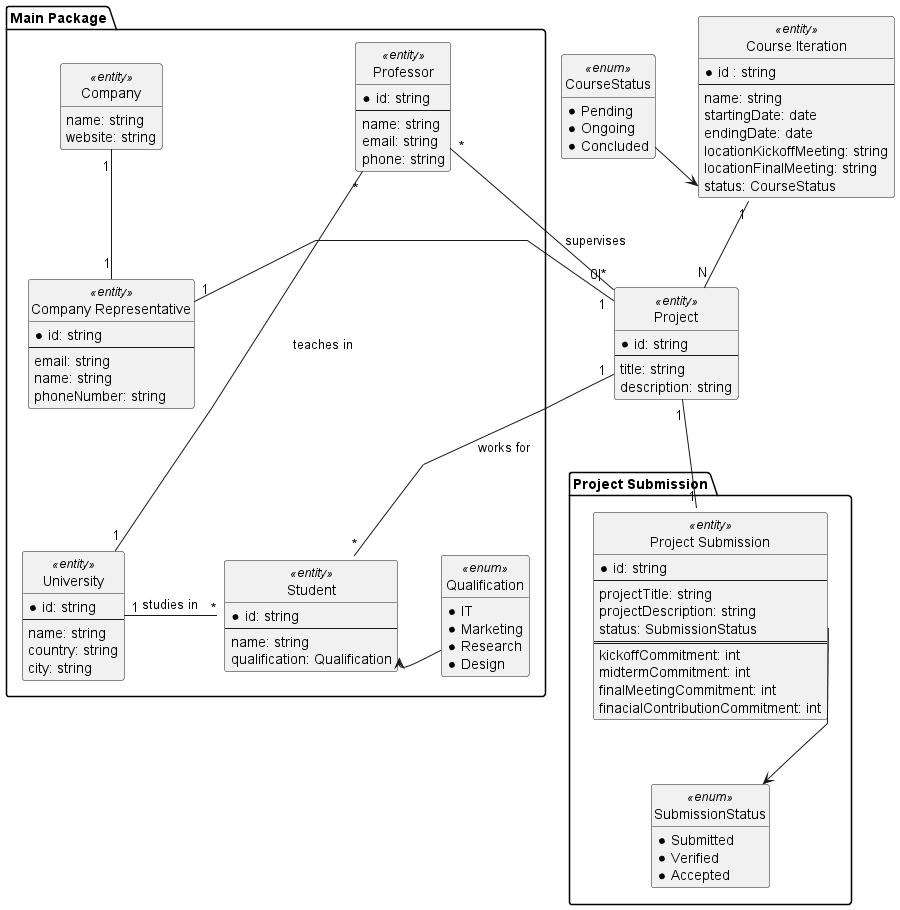
\includegraphics[width=\linewidth]{capitulos/cap3-analisedoproblema/assets/domain-diagram/dd.png}
    \caption{Diagrama de classes da lógica de negócio do Blended4Future 1}
    \label{fig:dd}
\end{figure}


A figura \ref{fig:dd} refere-se ao diagrama finalizado que foi definido.

\section{Engenharia de requisitos}

A Engenharia de Requisitos é uma área da Engenharia de Software que se dedica à identificação, análise, especificação, validação e gestão das necessidades e expectativas das partes interessadas relativamente a um sistema, com o objetivo de transformar essas necessidades, muitas vezes vagas ou incompletas, em requisitos claros, compreensíveis e verificáveis.

Esta secção dedica-se à apresentação dos requisitos estabelecidos para o sistema no arranque do projeto. 
Para uma melhor organização, estes requisitos foram divididos em dois grupos distintos: funcionais, que descrevem as operações fundamentais que a aplicação deve garantir, e não funcionais, que representam as condições e restrições que asseguram o correto desempenho dessas operações.


\subsection{Requisitos funcionais}
\label{subsection:requisitos_funcionais}

Durantes os primeiros dois sprints, junto dos professores, foi estabelecido um \textit{backlog} de \textit{user stories} que refletia a experiência desejada dos atores. 

A tabela \ref{tab:req-funcionais} reflete esta decisão.
\subsubsection{Diagrama de \textit{User Flow}}

Um Diagrama de \textit{User Flow} é uma representação visual que descreve o caminho que um utilizador percorre em um sistema ou aplicação para atingir um objetivo específico. Para uma melhor experiência de desenvolvimento, um destes foi elaborado. Este pode ser encontrado no anexo \ref{app:userflowchart}.    

\subsection{Requisitos não Funcionais}

\subsubsection{FURPS}
Para organizar e clarificar os requisitos do sistema, recorreu-se ao modelo \textbf{FURPS}, que permite classificar os requisitos em cinco categorias: 

\paragraph{Functionality (Funcionalidade)}
\begin{itemize}
    \item Funcionalidades de backoffice e frontoffice asseguradas com a respetiva autenticação.
\end{itemize}

\paragraph{Usability (Usabilidade)}
\begin{itemize}
    \item Interface intuitiva e consistente, que siga as normas de design.
    \item Navegação simples, permitindo localizar facilmente projetos e conteúdos.
    \item Feedback visual claro sobre ações realizadas (erros, confirmações).
\end{itemize}

\paragraph{Reliability (Confiabilidade)}
\begin{itemize}
    \item Garantir que o programa se mantém ativo e disponível, mesmo na presença de erros e outras adversidades.
    \item Assegurar que novas versões são disponibilizadas sem prejudicar a persistência de informação na base de dados.
\end{itemize}

\paragraph{Performance (Desempenho)}
\begin{itemize}
    \item Resposta rápida da interface mesmo com múltiplos utilizadores.
\end{itemize}

\paragraph{Supportability (Suportabilidade)}
\begin{itemize}
    \item Código modular e documentado para facilitar manutenção futura.
    \item Facilita a adição de novas funcionalidades ou integração com outras ferramentas.
\end{itemize}


Algumas destes requisitos foram considerados como casos de uso do programa e adicionados à tabela referida no ponto \ref{subsection:requisitos_funcionais} para facilitar o processo de desenvolvimento (Ex.: UC38, que refere a criação de pipelines de \textit{deployment} de novas versões). A tabela \ref{tab:req-nao-funcionais} subscreve esta decisão.

\begin{landscape}
\begin{longtable}{lp{20cm}}
\hline
    \textbf{User Story} & \textbf{Título} \\ \hline
    \endfirsthead

    \hline
    \textbf{User Story} & \textbf{Título} \\ \hline
    \endhead

    US2 & Como Representante da Empresa, quero alterar facilmente os detalhes da minha empresa (logótipo, contactos, etc.) para que represente melhor a sua imagem \\ \hline
    US3 & Como Representante da Empresa, quero submeter facilmente um novo projeto \\ \hline
    US4 & Como Empresa, quero relatórios com os resultados dos meus projetos. \\ \hline
    US6 & Como Professor, quero poder aceitar novas ideias de projeto \\ \hline
    US7 & Como Professor, quero poder selecionar um estudante e ver mais detalhes sobre ele (área de especialização, experiência profissional, LinkedIn) \\ \hline
    US8 & Como Professor, quero enviar convites a estudantes para participarem em projetos de acordo com as suas qualificações e interesses \\ \hline
    US9 & Como Estudante, gostaria de saber quais as qualificações necessárias para me inscrever num projeto \\ \hline
    US11 & Como Representante da Universidade, gostaria de poder contactar a Blended para aderir ao programa \\ \hline
    US12 & Como Utilizador, quero poder pesquisar projetos com base em critérios específicos \\ \hline
    US13 & Como Utilizador, quero receber uma confirmação por email após o registo para saber que a minha conta foi criada com sucesso \\ \hline
    US14 & Como Utilizador, quero ver uma página inicial \\ \hline
    US15 & Como Utilizador, gostaria de iniciar sessão na minha conta, para poder aceder às minhas informações pessoais \\ \hline
    US17 & Como Administrador, quero adicionar novas empresas ao sistema com o respetivo site e logótipo, para que a sua parceria seja visível na plataforma \\ \hline
    US18 & Como Administrador, quero poder suspender ou desativar contas de utilizadores \\ \hline
    US19 & Como Administrador, quero poder adicionar e gerir as universidades no sistema \\ \hline
    US20 & Como Administrador, quero poder adicionar novos utilizadores ao sistema \\ \hline
    US21 & Como Administrador, quero eliminar publicações no blogue para que informação desatualizada ou incorreta possa ser removida \\ \hline
    US22 & Como Administrador, quero receber alertas caso um projeto esteja inativo durante demasiado tempo para poder acompanhar os participantes \\ \hline
    US23 & Como Administrador, quero agendar publicações no blogue com antecedência para que o conteúdo seja publicado no momento certo \\ \hline
    US24 & Como Professor, quero criar publicações no blogue para que anúncios e ideias possam ser partilhados com os visitantes \\ \hline
    US25 & Como Professor, quero editar as minhas publicações no blogue para que informação desatualizada ou incorreta possa ser atualizada \\ \hline
    US26 & Como Professor, quero carregar e gerir fotografias de grupo e testemunhos de cada projeto para que os visitantes possam ver imagens e feedback relevantes \\ \hline
    US27 & Como Blended4Future, quero avaliar como os estudantes evoluíram ao longo de todo o projeto \\ \hline
    US28 & Como Utilizador, quero poder ver uma página de apresentação para empresas (elevator pitch) \\ \hline
    US29 & Como Utilizador, quero poder ver uma página de apresentação para estudantes (elevator pitch) \\ \hline
    US30 & Como Utilizador, quero poder ver uma página de apresentação para universidades (elevator pitch) \\ \hline
    US31 & Como Empresa, quero compreender melhor a identidade visual do conteúdo que quero apresentar \\ \hline
    US32 & Como Empresa, quero ter uma boa presença de antigos e atuais alunos nas redes sociais \\ \hline
    US33 & Como Empresa, quero ter publicações automáticas nas redes sociais, para que a sua presença online seja consistente \\ \hline
    US34 & Como Empresa, quero compreender que tipo de conteúdo quero apresentar nas nossas plataformas de redes sociais \\ \hline
    US35 & Como Empresa, quero compreender melhor o impacto da Blended em todas as partes interessadas (estudantes, universidades, empresas) \\ \hline
    US36 & Como Empresa, quero seguir as orientações para encontrar um novo nome para o projeto Blended4Future \\ \hline
    US37 & Como Empresa, quero ter uma Análise SWOT para o Blended4Future, de modo a compreender o seu valor e o seu mercado \\ \hline

\caption{Lista de requisitos funcionais}
\label{tab:req-funcionais}
\end{longtable}
\end{landscape}


\begin{landscape}
\begin{longtable}{lp{15cm}}
    \hline
    User Case & Title \\ \hline
    \endfirsthead

    \hline
    User Story & Title \\ \hline
    \endhead

    \hline
    \endfoot

    \hline
    \endlastfoot

    UC1 & Como Administrador, quero ter um sistema automatizado para implementar toda a solução \\ \hline
    UC5 & Como Programador, quero documentação que descreva toda a solução de forma abrangente \\ \hline
    UC10 & Como Sistema, quero que os projetos passem automaticamente de "em curso" para "concluídos" com base nas datas de início e fim, para que os estados se mantenham atualizados \\ \hline
    UC16 & Como Administrador, quero que o sistema associe automaticamente os estudantes a um projeto específico \\ \hline
    UC38 & Como Equipa de Desenvolvimento, quero ter pipelines configurados para o deployment automático no website, tanto para o backend como para o frontend \\ \hline
    UC39 & Como Sistema, quero notificar automaticamente os utilizadores sobre prazos dos projetos para que se mantenham informados \\ \hline

\caption{Lista de requisitos não funcionais}
\label{tab:req-nao-funcionais}
\end{longtable}
\end{landscape}



\section{Arquitetura do sistema}


\subsection{Desenho do sistema}





\subsection{Nível 1 - Contexto}

\subsubsection{Diagrama Lógico}

Na figura \ref{fig:diagram-lvl1-logical} encontra-se o diagrama lógico de nível. Este mostra os componentes desta arquitetura com um alto nível de abstração. Apenas é possível ver a exposição de 3 tipos de página \textit{web} para vários tipos de utilizadores: não registado, registado e administradores.   

\begin{figure}[h!tbp]
    \centering
    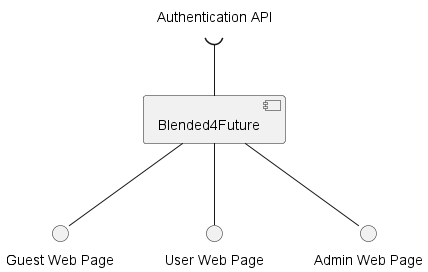
\includegraphics[width=0.5\linewidth]{capitulos/cap3-analisedoproblema/assets/arquiteturasistema/logical/logical_l1.png}
    \caption{Diagrama Lógico de Nível 1}
    \label{fig:diagram-lvl1-logical}
\end{figure}

\subsubsection{Diagrama Físico} 

A figura \ref{fig:diagram-lvl1-physical} demonstra o diagrama de físico de nível 1. Utiliza-se o \textit{port} 80 pois este é por norma utilizado em chamadas \Acrshort{HTTP} por este um protocolo baseado em \ACRshort{TCP}

\begin{figure}[h!tbp]
    \centering
    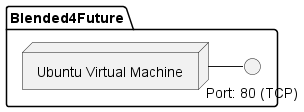
\includegraphics[width=0.5\linewidth]{capitulos/cap3-analisedoproblema/assets/arquiteturasistema/physical/physical_l1.png}
    \caption{Diagrama Físico de Nível 1}
    \label{fig:diagram-lvl1-physical}
\end{figure}





\subsection{Nível 2}

\subsubsection{Diagrama Lógico}

Na figura \ref{fig:diagram-lvl2-logical} é possivel ver um o anteriormente desmontrado na figura \ref{fig:diagram-lvl1-logical} com um menor nivel de abstração.
A este somam-se os conceitos de \textit{Frontend} e \textit{Backend}.

\begin{figure}[h!tbp]
    \centering
    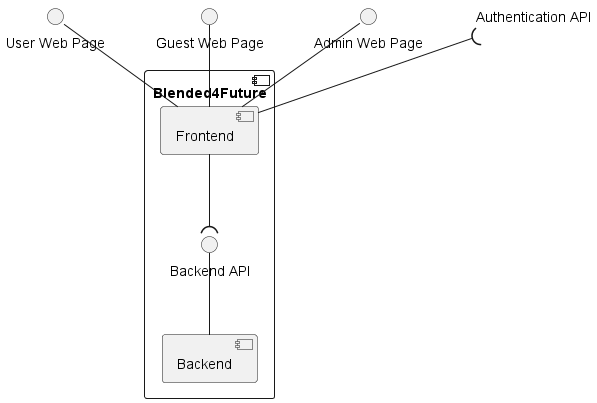
\includegraphics[width=0.7\linewidth]{capitulos/cap3-analisedoproblema/assets/arquiteturasistema/logical/logical_l2.png}
    \caption{Diagrama Lógico de Nível 2}
    \label{fig:diagram-lvl2-logical}
\end{figure}

\subsubsection{Diagrama de Implementação}

\subsubsection{Diagrama Físico} 

A figura \ref{fig:diagram-lvl2-physical} demonstra o diagrama de físico de nível 2. Neste entende-se a função do servidor \gls{NGINX} como a de criação de duas rotas para \textit{Backend} e \textit{Frontend}, respetivamente \textit{'/api'} e \textit{'/'}.

\begin{figure}[h!tbp]
    \centering
    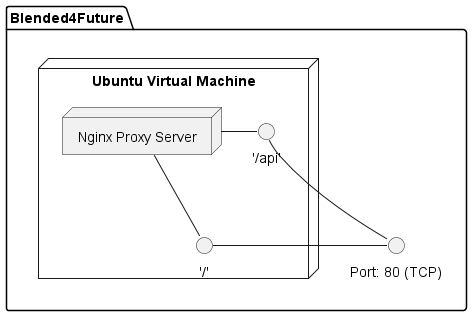
\includegraphics[width=0.6\linewidth]{capitulos/cap3-analisedoproblema/assets/arquiteturasistema/physical/physical_l2.png}
    \caption{Diagrama Físico de Nível 2}
    \label{fig:diagram-lvl2-physical}
\end{figure}




\subsection{Nível 3}

\subsubsection{Diagrama Lógico}

Com um nivel menor de abstração, a figura \ref{fig:diagram-lvl3-logical} apresenta aprofunda os modulos de \textit{Backend} e \textit{Frontend}. O primeiro é responsável pela logica de negócio e persistencia e, por tal, é detentor de uma aplicação Spring e de uma base de dados relacional \textit{MySQL}.

\begin{figure}[h!tbp]
    \centering
    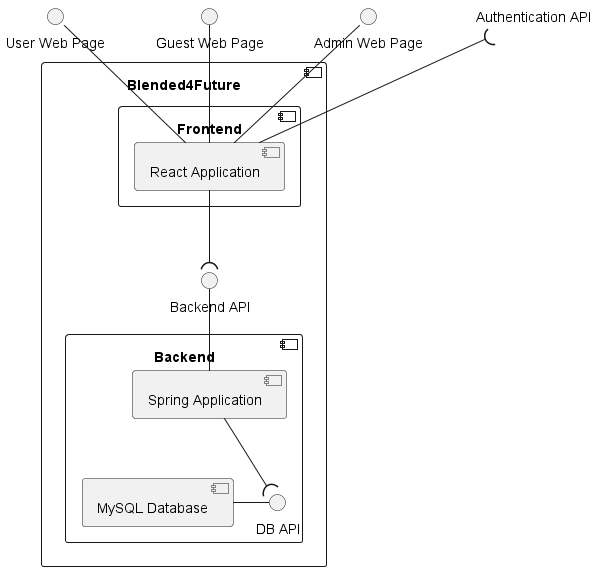
\includegraphics[width=0.8\linewidth]{capitulos/cap3-analisedoproblema/assets/arquiteturasistema/logical/logical_l3.png}
    \caption{Diagrama Lógico de Nível 3}
    \label{fig:diagram-lvl3-logical}
\end{figure}


\subsubsection{Diagrama de Implementação}

\subsubsection{Diagrama Físico} 
A figura \ref{fig:diagram-lvl3-physical} demonstra o diagrama de físico de nível 3. Com este é possível verificar o mapeamento das duas rotas criadas pelo servidor \textit{proxy} \gls{NGINX} para os PORTS 3000 e 4000, escolhidos, pois são memoráveis. Foi feita ainda a escolha de encapsular as aplicações \textit{Backend} e \textit{Frontend} em imagens \gls{Docker} garantindo assim o seu funcionamento independentemente do \textit{hardware} escolhido.

\begin{figure}[h!tbp]
    \centering
    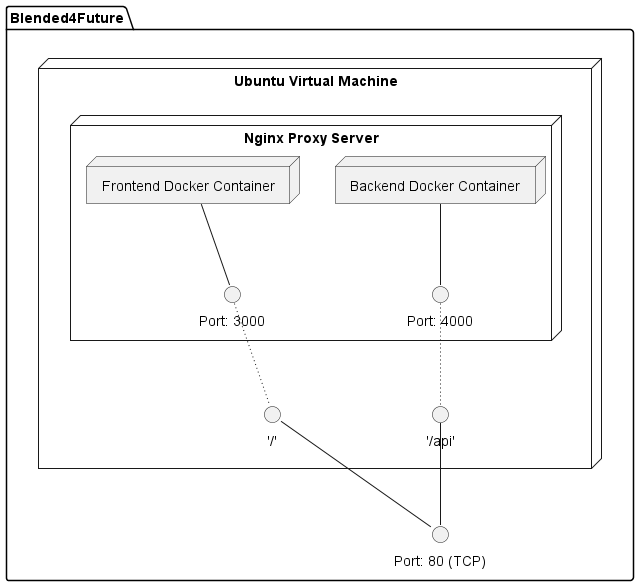
\includegraphics[width=0.7\linewidth]{capitulos/cap3-analisedoproblema/assets/arquiteturasistema/physical/physical_l3.png}
    \caption{Diagrama Físico de Nível 3}
    \label{fig:diagram-lvl3-physical}
\end{figure}





\subsection{Nível 4}

\subsubsection{Diagrama de Implementação}

\subsubsection{Diagrama Físico} 

A figura \ref{fig:diagram-lvl4-physical} demonstra o diagrama de físico de nível 4. Dento das respetivas imagens \gls{Docker} é possível as aplicações  \textit{Backend} e \textit{Frontend} encapsuladas. No contexto do \gls{Docker} é necessário fazer um mapeamento dos \textit{ports} utilizados do ambiente interno (Imagem) para o externo (Máquina Virtual), por isso é possível ver o mapeamento dos ports, respetivamente, internos e externos, 8080 e 4000, no \textit{Backend} e 3000 e 3000 no \textit{Frontend}.

Em nota, é possível incluir a base de dados na imagem graças à funcionalidade \textit{Volumes} do Docker e esta pode persistir diretamente no \textit{hardware} da máquina virtual.

\begin{figure}[h!tbp]
    \centering
    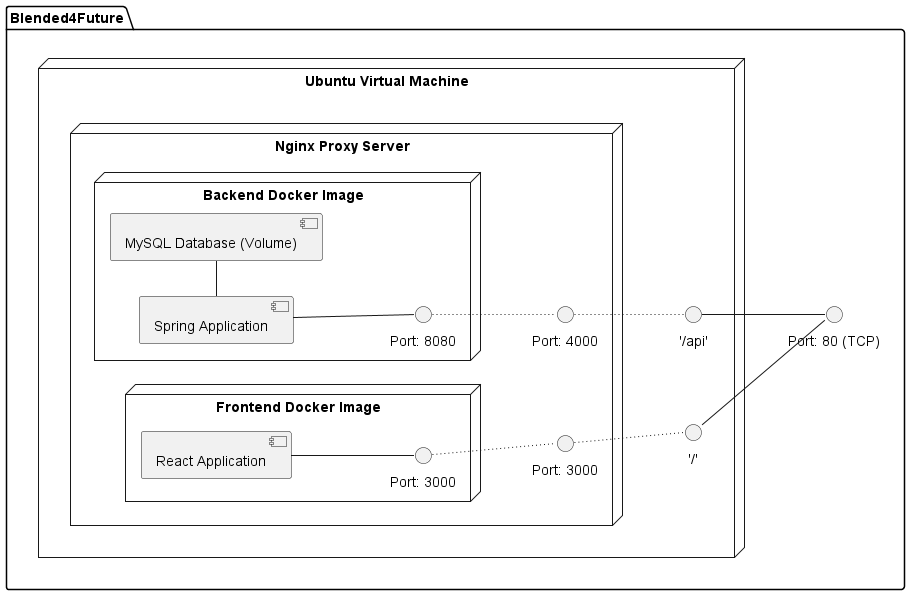
\includegraphics[width=\linewidth]{capitulos/cap3-analisedoproblema/assets/arquiteturasistema/physical/physical_l4.png}
    \caption{Diagrama Físico de Nível 4}
    \label{fig:diagram-lvl4-physical}
\end{figure}



\subsection{Padrões utilizados}


\chapter{Implementação de uma solução}

\section{A Implementação}

Este capitulo demonstrará a implementação de certas funcionalidades baseada na arquitetura apresentada anteriormente. Estas irão modulos de frontend, backend e as pipelines de deployment necessárias. 

\subsection{Backend}

O desenvolvimento do \textit{backend} constituiu uma das partes fundamentais do projeto, assegurando a implementação da lógica de negócio, a gestão dos dados e a comunicação entre o sistema e a interface de utilizador. Este componente atua como a camada central responsável por garantir que os processos internos sejam executados de forma consistente, segura e eficiente, proporcionando suporte às funcionalidades disponibilizadas no \textit{frontend}.  

Nesta secção irá se apresentar funcionalidades do backend no contexto da US3 (definida na tabela \ref{tab:req-funcionais}).







\subsubsection{Spring}
\label{sec:backend-Spring}

A framework Spring apresentou à equipa uma alta curva de aprendizagem. Os vários conceitos e ferramentas nesta são bastante alienígenas a qualquer outra ferramenta antes utilizada pelos membros. Por tal foi necessário mais tempo para a aprender. Alguns dos conceitos-chave considerados incluem:

\begin{itemize}
    \item \textbf{\textit{Spring Data}} é um agregado de módulos Spring que têm como função principal facilitar a programção de entidades e o seu respetivos acesso quando conectado a uma fonte de dados.

    \item \textbf{\textit{Spring Data JPA}} (ou só \textit{JPA}) é um dos módulos pertencente à coletânea Spring Data. O seu objetivo é facilitar a implementação de repositórios, reduzindo estes a interfaces Java, nas quais o Spring analisa o nome do método e implementa em \textit{runtime} o mesmo. 

    \item \textbf{\gls{Hibernate}} \cite{docs-hibernate} é uma framework Java e uma solução \ACRshort{ORM} que serve como implementação do \textit{JPA} para, logicamente, persistir a informação na respetiva base de dados.

    \item \textbf{\ACRshort{IoC}} (\acrlong{IoC}, em português \textit{Inversão de Controlo}) é um princípio de engenharia de \textit{software} que transfere a responsabilidade pela criação e gestão dos objetos para uma \textit{framework} específica. No \textit{Spring}, esta funcionalidade é desempenhada pelo denominado \textit{\ACRshort{IoC} Container}.
    
    \item \textbf{\textit{Bean}} corresponde a uma instância de objeto gerida pelo \textit{\ACRshort{IoC} Container}. Cada \textit{Bean} é criado, configurado e mantido pelo próprio contentor, segundo a configuração definida.
    
    \item \textbf{\ACRshort{DI}} (\acrlong{DI}, em português \textit{Injecção de Dependências}) é um princípio amplamente utilizado no desenvolvimento de \textit{software} que visa reduzir o acoplamento entre classes. No contexto do \textit{Spring}, esta prática é suportada através do \textit{IoC Container}, que fornece e gere as instâncias necessárias sob a forma de \textit{Beans}.
    
\end{itemize}









\subsubsection{Estrutura de pastas}

A estrutura de pastas do backend foi definida para enaltecer a função de cada ficheiro e/ou classe em cada uma, como pode ser observado na figura \ref{fig:folder-struct-backend}.

\begin{figure}
    \centering
    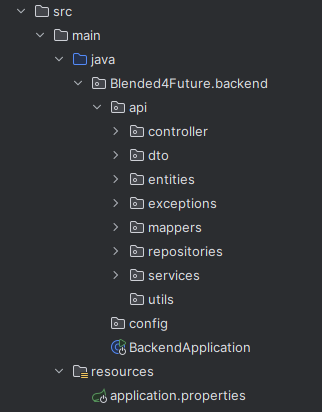
\includegraphics[width=0.5\linewidth]{capitulos/cap4-implementacao/assets/fold-struct-backend.png}
    \caption{Estrutura de pastas do backend}
    \label{fig:folder-struct-backend}
\end{figure}

\subsubsection{Entidades e relações}

Para o caso de uso a ser considerado, a entidade de maior importância será \textit{Project}. Esta encontra-se representada na figura \ref{fig:classe-projeto}.

Em nota, interessante enaltecer o uso das respetivas anotações:

\begin{itemize}
    \item \textbf{\textit{@Entity}} informa o \ACRshort{JPA}/\gls{Hibernate} que esta é uma entidade que deve ser persistida. Para tal deve conter um argumento anotado \lstinline|@Id|.
    \item \textbf{\textit{@Data}}\cite{docs-annotation-data} serve como substituto para as anotações \lstinline|@ToString|, \lstinline|@EqualsAndHashCode|, \lstinline|@Getter|, \lstinline|@Setter| e \lstinline|@RequiredArgsConstructor| que, respetivamente: 
    
    \begin{itemize}
        \item implementa o método \lstinline|toString()| incluindo todos os parâmetros não estáticos da classe;
        \item implementa o método \lstinline|equals(Object object)| e \lstinline|hashCodeO()|. Uma definição (\lstinline|callSuper|) teve de ser subscrita, pois era desejado inclusão dos atributos da superclasse \lstinline|BaseEntity| neste método (ver secção \ref{sec:base-entity});
        \item implementa métodos \textit{getter} para todos os atributos privados
        \item implementa metodos \textit{setter} para todos os atributos privados
        \item implementa um construtor com um parâmetro por atributo não final da classe.
    \end{itemize}

\end{itemize}


\begin{figure}
    \centering
    
    \begin{lstlisting}[language=Java]

@Entity
@Data
@EqualsAndHashCode(callSuper = true)
public class Project extends BaseEntity {

    @Column(nullable = false)
    @Convert(converter = ProjectName.NameConverter.class)
    private ProjectName name = new ProjectName();

    @Column(nullable = false)
    @Convert(converter = ProjectDescription.DescriptionConverter.class)
    private ProjectDescription description = new ProjectDescription();

    @ManyToOne
    private Company company;

    @ManyToOne
    private CompanyRepresentative companyRepresentative;

    @ManyToMany
    private Set<Student> students = Set.of();

    @ManyToMany
    private Set<Qualification> qualifications = Set.of();

    @OneToMany(mappedBy = "project", cascade = CascadeType.REMOVE)
    private Set<Report> reports = Set.of();

    @ManyToOne
    private CourseEdition courseEdition;
}

    \end{lstlisting}

    \caption{Classe \textit{Project}}
    \label{fig:classe-projeto}
\end{figure}













\subsubsection{\textit{BaseEntity}}
\label{sec:backend-base-entity}

Como medida de segurança e de padronização, foi desenvolvida a classe \textit{BaseEntity} (ver listagem \ref{lst:backend-base-entity}). Esta classe define dois identificadores: um interno e um externo. O identificador externo é utilizado na comunicação com o cliente, sendo retornado nos pedidos sob a forma de \textit{DTO}, enquanto o identificador interno é reservado para uso exclusivo do sistema.

Tal como o próprio nome indica, a \textit{BaseEntity} foi concebida para servir como \textit{superclasse} de todas as entidades persistentes.

A implementação da \textit{BaseEntity} envolve várias decisões de \textit{design} que merecem atenção:

\begin{itemize}
    \item No \gls{Hibernate}, os atributos definidos em superclasses não são, por defeito, persistidos. A utilização da anotação \lstinline|@MappedSuperclass| assegura que as classes filhas possam herdar esses parâmetros, permitindo a sua correta persistência na base de dados.

    \item A anotação \lstinline|@Id| define o atributo \lstinline|iid| como identificador principal da entidade no contexto da persistência. Complementarmente, \lstinline|@GeneratedValue(strategy=GenerationType.UUID)| especifica a forma como o identificador deve ser gerado, recorrendo ao padrão \textit{UUID}. Esta opção é particularmente relevante dado que, por omissão, o \gls{Hibernate} apenas consegue popular atributos de tipos primitivos.
    
    \item Verificou-se a necessidade de avaliar, de forma global, todos os atributos relacionados com a lógica de negócio, de modo a identificar e retornar eventuais erros existentes. Para esse fim, a função \lstinline|isBusinessDataValid()| analisa todos os \textit{Value Objects} (Ver secção \ref{sec:backend-value-objects}) da respetiva classe e devolve um \lstinline|HashMap| contendo a listagem dos erros detetados.
\end{itemize}

\begin{lstlisting}[language=Java,caption={Classe \textit{BaseEntity}},label={lst:base-entity}]
@MappedSuperclass
@Getter
public abstract class BaseEntity {

    @Id
    @GeneratedValue(strategy = GenerationType.UUID)
    private UUID iid;

    @Column(name="eid", unique = true, nullable = false)
    private UUID externalId;

    public BaseEntity() {
        this.externalId = generateCode();
    }

    private UUID generateCode() {
        return UUID.randomUUID();
    }

    public HashMap<String, Object> isBusinessDataValid() {

        HashMap<String, Object> errors = new HashMap<>();

        Class<?> clazz = this.getClass();
        List<IValueObject<?>> valueObjects = new ArrayList<>();

        while (clazz != null && clazz != Object.class) {
            for (Field field : clazz.getDeclaredFields()) {
                field.setAccessible(true);
                try {
                    Object value = field.get(this);

                    if (value instanceof IValueObject<?> vo) {
                        valueObjects.add(vo);
                    }
                } catch (IllegalAccessException ignored) {}
            }
            clazz = clazz.getSuperclass();
        }

        return isBusinessDataValid(valueObjects);
    }

    public static HashMap<String, Object> isBusinessDataValid(List<IValueObject<?>> fields) {
        HashMap<String, Object> errors = new HashMap<>();
        for (IValueObject<?> field : fields) {
            if (field == null) {
                continue;
            }
            errors.putAll(field.isValid());
        }
        return errors;
    }
}

\end{lstlisting}












\subsubsection{\textit{Value Objects}}
\label{sec:backend-value-objects}

A utilização de \textit{Value Objects} permite um maior controlo sobre a lógica de negócio inerente ao projeto. Por tal a sua implementação é necessária aquando a construção de um sistema de superior complexidade. 

A listagem \ref{lst:interface-value-object} mostra a interface \lstinline|ValueObject|.

\begin{lstlisting}[language=Java,caption={Interface \textit{Value Object}},label={lst:interface-value-object}]
public interface IValueObject<T> {
    T getValue();
    public HashMap<String, Object> isValid();
}
\end{lstlisting}

A notar, a função \lstinline|isValid()| em conjunto com a superclasse \lstinline|BaseEntity| permite verificar a lógica de negócio de cada respetivo \lstinline|ValueObject|. Para tal basta implementação fazer uma verificação do objecto em questão e retornar um \lstinline|HashMap| com toda a informação de erros.

\begin{lstlisting}[language=Java,caption={Classe \textit{ProjectDescription}},label={lst:class-project-description}]
@Value
public class ProjectDescription implements IValueObject<String> {

    public static final int MIN_LENGTH = 10;
    public static final int MAX_LENGTH = 500;
    public static final String DEFAULT_DESCRIPTION = "Default Project Description";

    private String description;

    @Override
    public String getValue() {
        return this.description;
    }

    public ProjectDescription(String value) {
        this.description = value;
    }

    public ProjectDescription() {
        this(DEFAULT_DESCRIPTION);
    }

    @Override
    public HashMap<String, Object> isValid() {
        HashMap<String, Object> errors = new HashMap<>();
        if (this.getValue() == null || this.getValue().isEmpty()) {
            errors.put("description", "Description cannot be null or empty");
        } else if (this.getValue().length() < MIN_LENGTH || this.getValue().length() > MAX_LENGTH) {
            errors.put("description", "Description must be between 10 and 500 characters long");
        }
        return errors;
    }

    @Converter
    public static class DescriptionConverter implements jakarta.persistence.AttributeConverter<ProjectDescription, String> {
        @Override
        public String convertToDatabaseColumn(ProjectDescription description) {
            return description.getValue();
        }

        @Override
        public ProjectDescription convertToEntityAttribute(String dbData) {
            return new ProjectDescription(dbData);
        }
    }
}
\end{lstlisting}

A listagem \ref{lst:class-project-description} demonstra uma implementação de \lstinline|IValueObject|. Como referido a função \lstinline|isValid()| avalia se o objeto é valido ou não retornando quaisquer erros.

Importante também seria referir a necessidade de um conversor, uma classe que informa o \gls{Hibernate} como deve mapear o objeto do programa para a base de dados e vice-versa.







\subsubsection{Repositórios}

Como referido na secção \ref{sec:backend-Spring}, o modulo Spring Data \ACRshort{JPA}, permite a implementação de repositórios em \textit{runtime}.

Tendo em conta a implementação de \lstinline|BaseEntity| e a necessidade de diferenciação entre identificadores internos e externos, foi implementada a interface \lstinline|BaseRepository| (ver listagem \ref{lst:interface-base-repository}). 

Na referida interface o uso de \lstinline|@NoRepositoryBean| informa o \ACRshort{IoC} \textit{Container} para não guardar uma instância deste repositório, pois por norma todos os \lstinline|JpaRepository| são guardados automaticamente. É ainda adicionada a função \lstinline|findByExternalId|, esta procura automaticamente por todas a instâncias que o correspondem ao nome do atributo \lstinline|externalId|. Esta segue uma nomenclatura especifica do Spring \cite{docs-spring-repository}.

\begin{lstlisting}[language=Java,caption={Inteface BaseRepository}, label={lst:interface-base-repository}]
@NoRepositoryBean
public interface BaseRepository<T extends BaseEntity> extends JpaRepository<T, UUID> {
    Optional<T> findByExternalId(UUID internalId);
}
\end{lstlisting}

Graças ao \gls{Spring} é possível então fazer implementações de repositórios muito facilmente, como exemplificado na listagem \ref{lst:interface-project-repository}

\begin{lstlisting}[language=Java, caption={interface \textit{ProjectRepository}}, label={lst:interface-project-repository}]
    public interface ProjectRepository extends BaseRepository<Project> {}
\end{lstlisting}







\subsubsection{Controladores e prevenção de erros}

Na eventualidade da ocorrência de erros, que estes sejam de negócio ou de sistema torna-se necessária implementar um sistema que os consiga detetar e retornar num formata predefinido, algo que o \gls{Spring} não faz por base. 

O \gls{Spring} disponibiliza \lstinline|@RestControllerAdvice| que permite a implementação de rotas ou ferramentas de deteção de erros em todas as classes anotadas com \lstinline|@RestController|.

Na listagem \ref{lst:class-AppExceptionController} entende-se o elemento base que permite capturar erros internos ou de negócio e retorná-los num formato predefinido (ver listagem \ref{lst:class-Error}). Em prática a anotação \lstinline|@ExceptionHandler(AppException.class)| faz com que a qualquer ponto de execução do programa, no caso de ser lançada uma exceção do tipo \lstinline|AppException| a esta se redirecione para a função \lstinline|handleAppException|. Na listagem \ref{lst:class-ProjectController} e \ref{lst:exception-AppException} mostra-se, respetivamente, exemplo do uso desta exceções e propria exceção \lstinline|AppException|.

\begin{lstlisting}[language=Java, caption={Class \textit{AppExceptionController}}, label={lst:class-AppExceptionController}]
@Slf4j
@RestControllerAdvice
@RequiredArgsConstructor
public class AppExceptionController {

    // Everytime an app exception is thrown, this method will be called
    // It will log the error and return a ResponseEntity with the error details
    @ResponseBody
    @ExceptionHandler(AppException.class)
    public ResponseEntity<?> handleAppException(AppException e, HttpServletRequest request) {
        log.error("App Exception occurred: {}", e.getMessage(), e);
        return createResponseError(e, request.getRequestURI());
    }

    private ResponseEntity<ErrorResponse> createResponseError(AppException e, String path) {
        Error err = new Error(
                e.getMessage(),
                e.getStatus().value(),
                path,
                Instant.now(),
                e.getData()
        );

        ErrorResponse errorResponse = ErrorResponse.fromError(err);

        return new ResponseEntity<>(errorResponse,new HttpHeaders(), e.getStatus());
    }

}
\end{lstlisting}

\begin{lstlisting}[language=Java, caption={Class \textit{Error}}, label={lst:class-Error}]
@Value
@AllArgsConstructor(access = PUBLIC)
public class Error {
    String message;
    int status;
    String path;
    Instant timestamp;
    Map<String, Object> data;
}
\end{lstlisting}

\begin{lstlisting}[language=Java, caption={Class \textit{ProjectController}}, label={lst:class-ProjectController}]
@RestController
@RequestMapping("/api/project")
public class ProjectController {


    private final IProjectService service;

    public ProjectController(IProjectService IProjectService) {
        this.service = IProjectService;
    }

    @GetMapping("")
    public List<ProjectDTO> getAllProjects() {
        return service.getProjects();
    }

    @GetMapping("/{id}")
    public ProjectDTO getProjectById(UUID id) {
        try {
            return service.getProject(id);
        } catch (NoSuchElementException e) {
            throw new AppException(e, HttpStatus.NOT_FOUND);
        }
    }

    @PostMapping("")
    public ProjectDTO addProject(@RequestBody AddProjectDTO project) {
        try {
            return service.addProject(project);
        } catch (NoSuchElementException e) {
            throw new AppException(e, HttpStatus.NOT_FOUND);
        } catch (FormDataException e) {
            throw new AppException(e, HttpStatus.BAD_REQUEST, e.getErrors());
        }
    }

    @PutMapping("/{id}")
    public ProjectDTO updateProject(@PathVariable UUID id, @RequestBody @Valid AddProjectDTO project) {
        try {
            return service.updateProject(id, project);
        } catch (NoSuchElementException e) {
            throw new AppException(e, HttpStatus.NOT_FOUND);
        } catch (FormDataException e) {
            throw new AppException(e, HttpStatus.BAD_REQUEST, e.getErrors());
        }
    }

    @DeleteMapping("/{id}")
    public ProjectDTO deleteProject(@PathVariable UUID id) {
        try {
            return service.deleteProject(id);
        } catch (NoSuchElementException e) {
            throw new AppException(e, HttpStatus.NOT_FOUND);
        }
    }
}
\end{lstlisting}

\begin{lstlisting}[language=Java, caption={Exceção \textit{AppException}}, label={AppException}]
@Getter
public class AppException extends RuntimeException{

    private final HttpStatus status;
    private Map<String, Object> data;

    public AppException(String message, HttpStatus status, Map<String, Object> data) {
        super(message);
        this.status = status;
        this.data = data;
    }

    public AppException(Exception e, HttpStatus status, Map<String, Object> data) {
        super(e.getMessage());
        this.status = status;
        this.data = data;
    }

    public AppException(Exception e, HttpStatus status) {
        super(e.getMessage());
        this.status = status;
        this.data = new HashMap<>();
    }

    public AppException(String message, HttpStatus status) {
        super(message);
        this.status = status;
        this.data = new HashMap<>();
    }
}
\end{lstlisting}

\subsection{Frontend}

\subsubsection{Paginas Estáticas}

\subsubsection{Pagina de Visualização de Projetos}



\subsection{Controlo de Versões}

Em todos os repositórios em uso foi definido o uso de multiplos \textit{branches}, tendo como principais o \textit{main/master} e o \textit{dev}. 

Para o desenvolvimento de qualquer nova funcionalidade era necessário a criação de um novo branch baseado na versão mais recente do \textit{dev}. Quando este era finalizado era feito um \textit{merge} devolta no mesmo. Aquando da necessidade de lançar uma nova versão bastava dar merge da versão desejada do \textit{dev} no branch \textit{main}.




\subsection{Deployments}

Como foi explicado anteriormente, um dos requisitos definidos  era a criação de um ambiente de \textit{CI/CD} que permitisse simplicar o processo de desenvolvimento, facilitando a disponibilização de novas versões.

A plataforma Azure disponbiliza a funcionalidade \textit{Pipelines}. Com o recurso à linguagem YAML, esta permite definir os trabalhos que os "agentes" definidos pelo utilizador

Finalmente, utilizando a ferramenta Docker é possível "empacotar" o código numa só unidade que funciona de forma igual em diferentes máquinas. Esta funcionalidade será feita numa màquina Linux Ubuntu 24.04.2. 

\subsubsection{Definição dos agentes}

No contexto do Azure Pipelines um agente (em inglês, \textit{Agent}) é a maquiná indica ao Azure Pipelines que executará os trabalhos pedidos, como por exemplo compilar o projeto. 

Neste caso iremos indicar ao Azure Pipelines para que utilize a nossa máquina como um agente. O agente irá executar dentro de um \textit{container Docker}.

A Microsoft oferece ferramentas para ajudar neste processo \cite{run-a-self-hosted-agent-in-docker}. O script que estabelece a relação entre os agentes e os serviços Azure, tal como o Dockerfile necessário para a compilção do Docker poderá ser encontrado nos anexos \ref{app:pipeline-start.sh} e \ref{app:dockerfile-pipeline-agent} respetivamente.

Após a criação do agente basta iniciar o \textit{container Docker}, tendo em atenção à indicação das variaveis de ambiente necessárias. A figura \ref{fig:start-docker-agent} demonstra isso mesmo, com censura a qualquer informação sensivel à organização.

\begin{figure}[h!tbp]
    

\begin{lstlisting}
    sudo docker run -d 
        -e AZP_URL="https://dev.azure.com/blended4future2025" 
        -e AZP_TOKEN="******" 
        -e AZP_POOL="*******" 
        -e AZP_AGENT_NAME="*****" 
        --name "azp-agent-linux" 
        devops-agent:linux
\end{lstlisting}


\caption{Script de inicialização do Container Docker para o agente do Azure Pipelines}
\label{fig:start-docker-agent}

\end{figure}

Logo após, é possivél ver o agente disponível no Azure DevOps (Figura \ref{fig:agent-devops}). 

\begin{figure}[h!tbp]
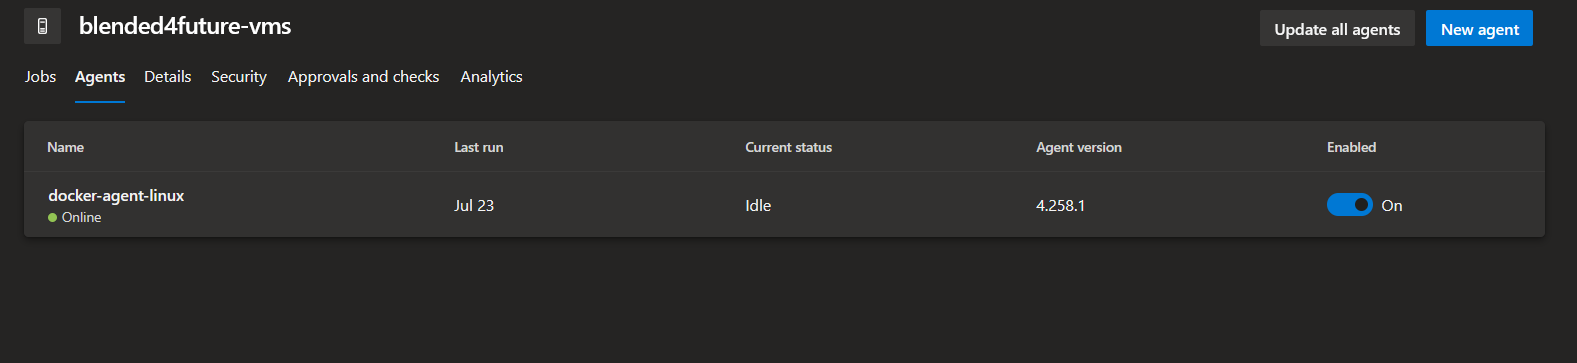
\includegraphics[width=\linewidth]{capitulos/cap4-implementacao/assets/devops-agent.png}
\caption{Agente disponbilizado no Azure DevOps}
\label{fig:agent-devops}
\end{figure}

\subsubsection{Trabalhos da pipeline}

O conceito de trabalho (em inglês, \textit{Job}) é de extrema importância no Azure Pipelines. Este premite definir ações e os seus resptivos passos para atingir um objetivo.

Nesta secção demonstra-se a \textit{pipeline} criada e os respetivos passos por ela tomados, utilizando como exemplo a definida para o módulo frontend. A versão completa deste ficheiro poderá ser encontrada no appêndice \ref{app:pipeline-yaml}. 

\begin{figure}[h!tbp]
    \centering
    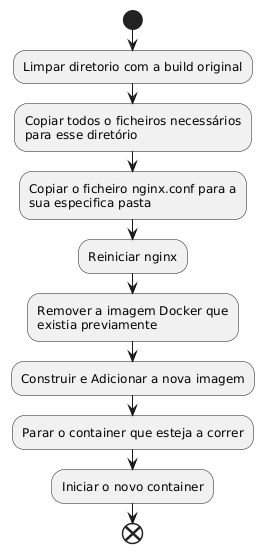
\includegraphics[width=0.3\linewidth]{capitulos/cap4-implementacao/assets/pipeline-activity-diagram.png}
    \caption{Diagrama de atividade representante da Pipeline de construção de uma nova versão}
    \label{fig:pipeline-ad}
\end{figure}


Na figura \ref{fig:pipeline-ad}, é possível ver o um diagrama de atividade que descreve cada passo feito por este trabalho.

\begin{lstlisting}[caption={Trigger - Pipeline},label={lst:pipeline-trigger}]
trigger:
    branches:
        include:
            - main
\end{lstlisting}


A listagem \ref{lst:pipeline-trigger}, descreve o gatilho (em inglês, \textit{trigger}) de ativação da pipeline. Neste caso qualquer \textit{commit} no \textit{branch} "main" irá ativar os trabalhos definidos.

É importante enaltecer que existem variáveis que foram definidas externamente através do Azure DevOps e que são utilizadas ao longo da pipeline. Estas são:

\begin{itemize}
    \item \textbf{CONTAINERNAME}: Nome que o \gls{Container} terá quando for criado.
    \item \textbf{FRONTENDBUILDPATH}: Caminho para o qual o projeto será copiado para.
    \item \textbf{VMBUILDPATH}: Caminho para o qual a \gls{Build} do projeto irá ser colada em.
\end{itemize}

Finalmente, cada passo segue o conceito apresentado na figura \ref{fig:pipeline-ad}. Especial atenção para o uso de \lstinline|SSH@0|\cite{docs-SSH0}, esta é uma task pre disponbilizada para estabelecer uma conexção SSH a uma màquina alvo. A chave está definida como segredo e é importado no início do ficheiro quando ocorre uma referência ao grupo de variáveis "ssh".



\section{Testes}

A prática de testes é fundamental para assegurar o correto funcionamento de qualquer programa, permitindo verificar se o código implementado cumpre as especificações definidas. Esta secção pretende apresentar e detalhar os diferentes tipos de testes realizados ao longo do projeto e as tecnologias utilizadas para este.

\subsection{Testes Unitários}

Os testes unitários constituem uma prática essencial no desenvolvimento de \textit{software}, cujo principal objetivo é garantir que cada unidade de código se comporta conforme esperado. Esta abordagem permite a deteção precoce de erros, aumenta a fiabilidade do \textit{software} e facilita a manutenção e evolução do sistema. Para a execução destes testes, deu-se prioridade à utilização do \textit{JUnit}, em conjunto com as ferramentas disponibilizadas pelo \gls{Spring}.

A Figura \ref{lst:class-CompanyTest} apresenta um exemplo de teste unitário que valida a correta criação de um objeto \lstinline|Company| e a sua inserção no \lstinline|entityManager|, permitindo a persistência dos objetos diretamente em \textit{runtime}.

\begin{lstlisting}[language=Java, label={lst:class-CompanyTest}, caption={Class \textit{CompanyTest} - Exemplificação de testes Unitários}]
@DataJpaTest()
class CompanyTest {

    @Autowired
    private TestEntityManager entityManager;

    @Autowired
    private CompanyRepository companyRepository;

    @Test
    void shouldPersistAndLoadCompanyWithValueObjects() {
        Company company = new Company();
        company.setName(new CompanyName("OpenAI"));
        company.setDescription(new CompanyDescription("Artificial Intelligence Research"));

        entityManager.persist(company);
        entityManager.flush();
        entityManager.clear();

        Optional<Company> found = companyRepository.findById(company.getIid());

        assertThat(found.isEmpty()).isFalse();
        assertThat(found.get().equals(company));
    }
    |\Suppressnumber|
    ...
    |\Reactivatenumber|
}
\end{lstlisting}

Foram implementados testes unitários para as entidades de domínio, bem como para os respetivos \lstinline|ValueObjects|, abrangendo tanto casos de sucesso, com dados válidos, como casos de insucesso, com informações incorretas.

\subsection{Testes de Implementação}

Para os testes de implementação, deu-se especial ênfase à utilização da ferramenta Postman, a qual proporciona um ambiente colaborativo e estruturado para a testagem de \gls{API}.

A Listagem \ref{lst:postman-post-company} apresenta o \textit{script} pós-teste executado pelo \textit{postman} para verificar a resposta ao pedido do tipo POST para "/company". 

\begin{lstlisting}[style=Javascript, label={lst:postman-post-company}, caption={Script de test da rota POST /company}]
pm.test("Status code is 201", function () {
    pm.response.to.have.status(201);
});

pm.test("Response has correct company data", function () {
    var jsonData = pm.response.json();
    pm.expect(jsonData.name.value).to.eql("OpenAI");
    pm.expect(jsonData.description.value).to.eql("Artificial Intelligence Research");
    pm.expect(jsonData.id).to.exist;
})

const companyId = pm.response.json().id;
await pm.sendRequest({
    url: `${pm.environment.get("localhost")}/company/${companyId}`,
    method: 'DELETE',
    header: {
        'Content-Type': 'application/json'
    }
});
\end{lstlisting}





\section{Avaliação da solução}

\chapter{Reflexão sobre trabalho em equipa}

%----------------------------------------------------------------------------------------
%	BIBLIOGRAPHY
%----------------------------------------------------------------------------------------

\printbibliography[heading=bibintoc]

%----------------------------------------------------------------------------------------
%	THESIS CONTENT - APPENDICES
%----------------------------------------------------------------------------------------
% Include the appendices of the thesis as separate files from the Appendices folder
% Uncomment the lines as you write the Appendices
\begin{appendices}

% Appendix A

\chapter{Appendix Title Here} % Main appendix title

\label{AppendixA} % For referencing this appendix elsewhere, use \ref{AppendixA}

Write your Appendix content here.
%\input{appendices/appendixB}
%\input{appendices/appendixC}

\end{appendices}
%----------------------------------------------------------------------------------------

\end{document}
